% ---
% title: KKT reviews
% date: 2026-04-22
% tag: Math
% excerpt: 隔了两周再翻 KKT：原始可行性、对偶可行性、驻点和互补松弛，逐条对上几何直觉，再回头看约束规范。
% ---
\section{经典带约束优化问题回顾}

\href{https://zhuanlan.zhihu.com/p/556931657}{信息来源·知乎}

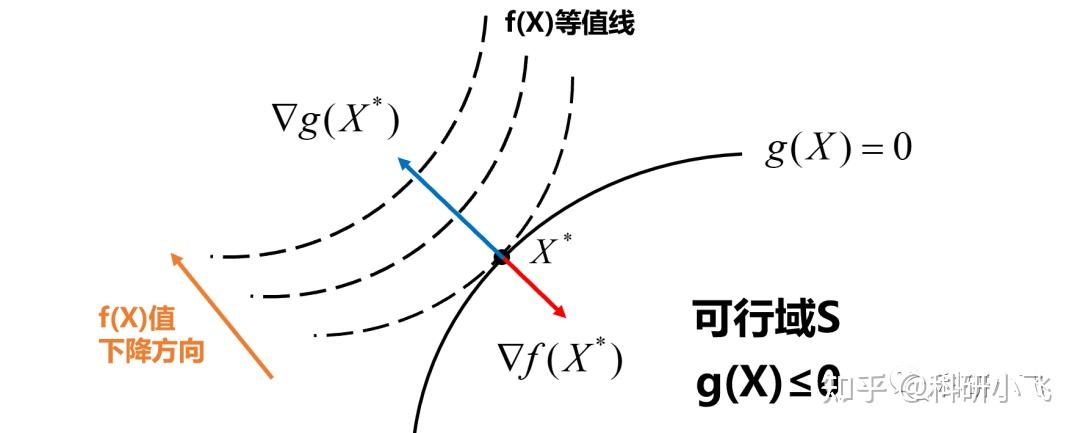
\includegraphics[width=0.50\linewidth]{notes/assets/v2-052b0104b46e31fa4d7a05e9c6f3d2b5_1440w.jpg}


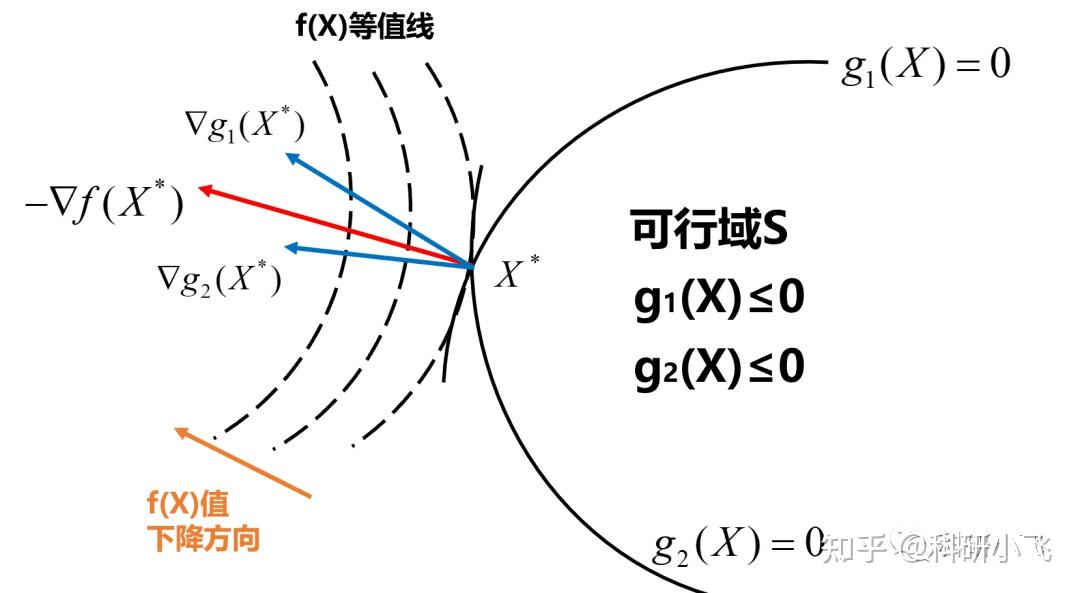
\includegraphics[width=0.50\linewidth]{notes/assets/v2-978615fba2aa975e0f4f7f28fdfbc103_1440w.jpg}

\subsection{Karush–Kuhn–Tucker Conditions（KKT 条件）}

KKT 条件给出带约束优化问题的一阶最优性条件，可以看作无约束情形“梯度为零”的推广。

在适当的正则性条件（constraint qualification）下，局部最优解 \(x^*\) 满足一组关于目标函数、约束函数和拉格朗日乘子的条件，这就是 KKT 条件。

\section{标准优化问题}

考虑如下优化问题：

\[
\begin{aligned}
\min_{x \in \mathbb{R}^n} \quad & f(x) \\
\text{s.t.} \quad 
& g_i(x) \le 0, \quad i=1,\dots,m,\\
& h_j(x) = 0, \quad j=1,\dots,l.
\end{aligned}
\]

其中 \(f(x)\) 是目标函数，\(g_i(x)\) 是不等式约束，\(h_j(x)\) 是等式约束。

我们称满足所有约束的点 \(x\) 为可行点（feasible point）。

\section{拉格朗日函数}

为处理约束，引入拉格朗日乘子：

\begin{itemize}
  \item \(\mu_i \ge 0\)：对应不等式约束 \(g_i(x)\le 0\)
  \item \(\nu_j \in \mathbb{R}\)：对应等式约束 \(h_j(x)=0\)
\end{itemize}

定义拉格朗日函数：

\[
\mathcal{L}(x,\mu,\nu)
=
f(x)
+
\sum_{i=1}^m \mu_i g_i(x)
+
\sum_{j=1}^l \nu_j h_j(x).
\]

\section{KKT 条件}

若 \(x^*\) 是局部最优解，并且满足适当的约束资格条件，则存在乘子 \(\mu^*\) 与 \(\nu^*\)，使得以下条件成立：

\subsection{原始可行性（Primal Feasibility）}

\[
g_i(x^*) \le 0,\quad i=1,\dots,m \\

h_j(x^*) = 0,\quad j=1,\dots,l
\]

即 \(x^*\) 本身必须是可行点。

\subsection{对偶可行性（Dual Feasibility）}

\[
\mu_i^* \ge 0,\quad i=1,\dots,m
\]

这是不等式约束乘子的符号条件。

\subsection{驻点条件（Stationarity）}

\[
\nabla f(x^*)
+
\sum_{i=1}^m \mu_i^* \nabla g_i(x^*)
+
\sum_{j=1}^l \nu_j^* \nabla h_j(x^*)
=0
\]

这相当于“带约束的一阶最优条件”。

\subsection{互补松弛（Complementary Slackness）}

\[
\mu_i^* g_i(x^*) = 0,\quad i=1,\dots,m
\]

若某个不等式约束不活跃（\(g_i(x^*)<0\)），对应的 \(\mu_i^*=0\)；若 \(\mu_i^*>0\)，则该约束必须活跃（\(g_i(x^*)=0\)）。

\section{KKT 条件的直观理解}

最优点不能沿可行方向继续下降，因此目标函数梯度必须能写成活跃约束梯度的线性组合。约束“挡住”了下降方向。

\section{何时 KKT 是必要条件？}

一般来说，KKT 条件是局部最优解的必要条件，但需要附加一定的正则性条件。
否则，即使 \(x^*\) 是最优点，也可能找不到满足 KKT 的乘子。

因此，正确的表述通常是：

\begin{quote}
在可微性与适当约束资格条件成立时，局部极小点满足 KKT 条件。
\end{quote}

\section{何时 KKT 也是充分条件？}

若问题是凸优化问题，则 KKT 条件不仅是必要的，也是充分的。

更具体地说，若：

\begin{itemize}
  \item \(f(x)\) 是凸函数
  \item 每个 \(g_i(x)\) 是凸函数
  \item 每个 \(h_j(x)\) 是仿射函数（线性函数加常数）
\end{itemize}

那么只要存在点 \(x^*\) 与乘子 \((\mu^*,\nu^*)\) 满足 KKT 条件，就可以断定：

\[
x^* \text{ 是全局最优解。}
\]

\section{约束资格条件（Constraint Qualification, CQ）}

KKT 成立通常需要额外的“正则性假设”，这些假设统称为约束资格条件。

\subsection{LICQ}

线性无关约束资格条件（Linear Independence Constraint Qualification）：在 \(x^*\) 处，所有活跃不等式约束的梯度与等式约束的梯度线性无关。

\subsection{MFCQ}

Mangasarian–Fromovitz Constraint Qualification。比 LICQ 更弱，是优化里常用的条件。

\subsection{CRCQ}

常秩约束资格条件（Constant Rank Constraint Qualification）要求某些约束梯度子集在邻域内保持秩不变。

\subsection{CPLD}

常正线性相关约束资格条件（Constant Positive Linear Dependence），比上面几类更弱。

\subsection{Slater 条件}

对于凸优化中的不等式约束问题，若存在某点 \(x\) 使得

\[
g_i(x) < 0,\quad \forall i=1,\dots,m,
\]

则称满足 Slater 条件。

Slater 条件保证 KKT 条件成立，也保证强对偶性。

\subsection{常见关系}

通常有如下蕴含关系：

\begin{verbatim}
graph TD
    A[LICQ] --> B[MFCQ]
    B --> C[CPLD]
    A --> D[CRCQ]
    D --> C
\end{verbatim}

也就是说：

\[
\mathrm{LICQ} \Rightarrow \mathrm{MFCQ} \Rightarrow \mathrm{CPLD}
\]

\[
\mathrm{LICQ} \Rightarrow \mathrm{CRCQ} \Rightarrow \mathrm{CPLD}
\]

一般来说，越弱的约束资格条件越容易满足，但能推出的结论也往往更弱。

\section{解题步骤总结}

做 KKT 题目时，通常按下面步骤走：

\begin{enumerate}
  \item 写出标准形式

  \begin{itemize}
    \item 目标函数
    \item 不等式约束写成 \(g_i(x)\le 0\)
    \item 等式约束写成 \(h_j(x)=0\)
  \end{itemize}
  \item 写拉格朗日函数
  \item 列 KKT 四组条件

  \begin{itemize}
    \item 原始可行性
    \item 对偶可行性
    \item 驻点条件
    \item 互补松弛
  \end{itemize}
  \item 判断哪些约束可能活跃
  \item 联立求解 \(x^*,\mu^*,\nu^*\)
  \item 若是凸问题，可直接得出全局最优
\end{enumerate}

\section{例题 1：只有不等式约束}

\subsection{题目}

求解：

\[
\begin{aligned}
\min_{x,y}\quad & x^2+y^2\\
\text{s.t.}\quad & 1-x-y\le 0
\end{aligned}
\]

\subsection{第一步：写拉格朗日函数}

设约束为

\[
g(x,y)=1-x-y\le 0
\]

拉格朗日函数为

\[
\mathcal{L}(x,y,\mu)=x^2+y^2+\mu(1-x-y)
\]

其中 \(\mu\ge 0\)。

\subsection{第二步：写 KKT 条件}

\subsubsection{驻点条件}

\[
\frac{\partial \mathcal{L}}{\partial x}=2x-\mu=0
\]

\[
\frac{\partial \mathcal{L}}{\partial y}=2y-\mu=0
\]

因此

\[
x=y=\frac{\mu}{2}
\]

\subsubsection{原始可行性}

\[
1-x-y\le 0
\]

\subsubsection{对偶可行性}

\[
\mu\ge 0
\]

\subsubsection{互补松弛}

\[
\mu(1-x-y)=0
\]

\subsection{第三步：求解}

由 \(x=y=\mu/2\)，代入互补松弛：

\[
\mu\left(1-\frac{\mu}{2}-\frac{\mu}{2}\right)=\mu(1-\mu)=0
\]

所以：

\begin{itemize}
  \item 若 \(\mu=0\)，则 \(x=y=0\)，但此时 \(1-0-0=1>0\)，不可行
  \item 因此只能有 \(\mu=1\)
\end{itemize}

于是：

\[
x^*=y^*=\frac12
\]

\subsection{结论}

最优解为

\[
\left(\frac12,\frac12\right)
\]

最优值为

\[
f(x^*)=\frac14+\frac14=\frac12
\]

\section{例题 2：只有等式约束}

\subsection{题目}

求解：

\[
\begin{aligned}
\min_{x,y}\quad & x^2+y^2\\
\text{s.t.}\quad & x+y-1=0
\end{aligned}
\]

\subsection{第一步：拉格朗日函数}

设等式约束为

\[
h(x,y)=x+y-1=0
\]

拉格朗日函数：

\[
\mathcal{L}(x,y,\nu)=x^2+y^2+\nu(x+y-1)
\]

\subsection{第二步：驻点条件}

\[
\frac{\partial \mathcal{L}}{\partial x}=2x+\nu=0
\]

\[
\frac{\partial \mathcal{L}}{\partial y}=2y+\nu=0
\]

因此

\[
x=y
\]

再结合约束

\[
x+y=1
\]

得到

\[
x^*=y^*=\frac12
\]

\hrule

\subsection{结论}

最优解为

\[
\left(\frac12,\frac12\right)
\]

最优值为

\[
\frac12
\]

这个结果也符合几何直觉：在直线 \(x+y=1\) 上，离原点最近的点就是 \(\left(\frac12,\frac12\right)\)。

\section{例题 3：混合约束}

\subsection{题目}

求解：

\[
\begin{aligned}
\min_{x,y}\quad & (x-1)^2+(y-2)^2\\
\text{s.t.}\quad & -x\le 0,\\
& 2-x-y\le 0
\end{aligned}
\]

即

\[
x\ge 0,\quad x+y\ge 2
\]

\subsection{第一步：拉格朗日函数}

设

\[
g_1(x,y)=-x\le 0,\qquad g_2(x,y)=2-x-y\le 0
\]

则

\[
\mathcal{L}(x,y,\mu_1,\mu_2)
=
(x-1)^2+(y-2)^2+\mu_1(-x)+\mu_2(2-x-y)
\]

其中

\[
\mu_1,\mu_2\ge 0
\]

\subsection{第二步：驻点条件}

\[
\frac{\partial \mathcal{L}}{\partial x}=2(x-1)-\mu_1-\mu_2=0
\]

\[
\frac{\partial \mathcal{L}}{\partial y}=2(y-2)-\mu_2=0
\]

\subsection{第三步：观察最优点是否在约束内部}

无约束最小点是

\[
(1,2)
\]

检查它是否可行：

\begin{itemize}
  \item \(x=1\ge 0\)
  \item \(x+y=3\ge 2\)
\end{itemize}

所以它本来就满足所有约束。

因此最优解实际上就是：

\[
x^* = 1,\qquad y^* = 2
\]

并且两个约束都不活跃：

\[
g_1(1,2)=-1<0,\qquad g_2(1,2)=-1<0
\]

由互补松弛可知：

\[
\mu_1^*=\mu_2^*=0
\]

\subsection{结论}

最优解为

\[
(1,2)
\]

这个例子说明：

\begin{quote}
若无约束极小点本身已经可行，那么所有不活跃约束的乘子都为零。
\end{quote}

\section{一个常见易错点}

\subsection{不等式方向必须统一}

KKT 的标准写法通常默认：

\[
g_i(x)\le 0
\]

所以遇到约束时，记得先统一符号。例如：

\begin{itemize}
  \item \(x+y\ge 1\) 应改写为
  
  \[
  1-x-y\le 0
  \]
  \item \(x\ge 0\) 应改写为
  
  \[
  -x\le 0
  \]
\end{itemize}

否则乘子的符号很容易写错。

\section{总结}

KKT 把最优点的判断拆成四类条件：原始可行性、对偶可行性、驻点条件和互补松弛。一般非线性规划里，它是局部最优的必要条件；凸优化里，它还是全局最优的充分条件。

学的时候要会两件事：列出条件，解释每个条件的几何和代数意义。

\section{附图}

\begin{center}
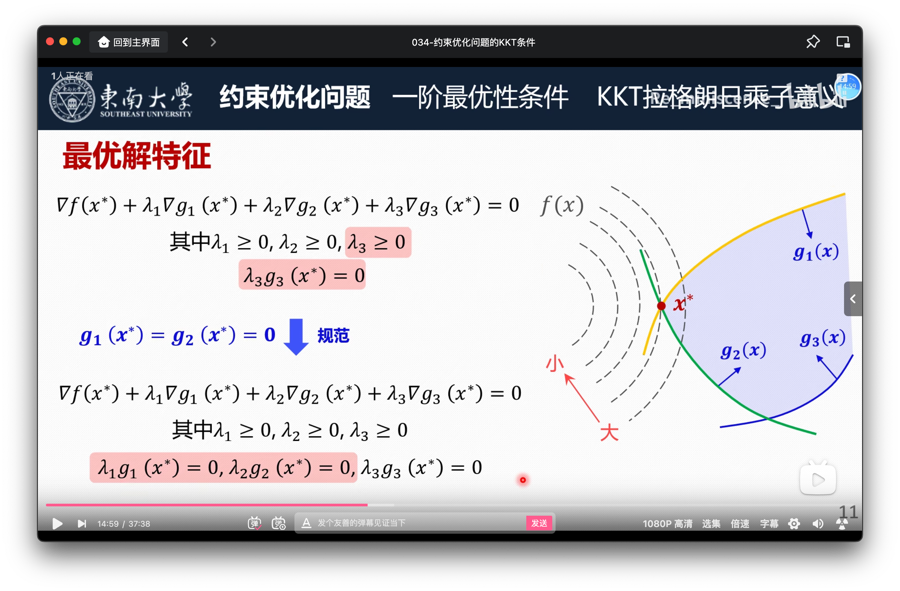
\includegraphics[width=0.50\linewidth]{notes/assets/image-20260107150143874.png}
\end{center}

\begin{center}
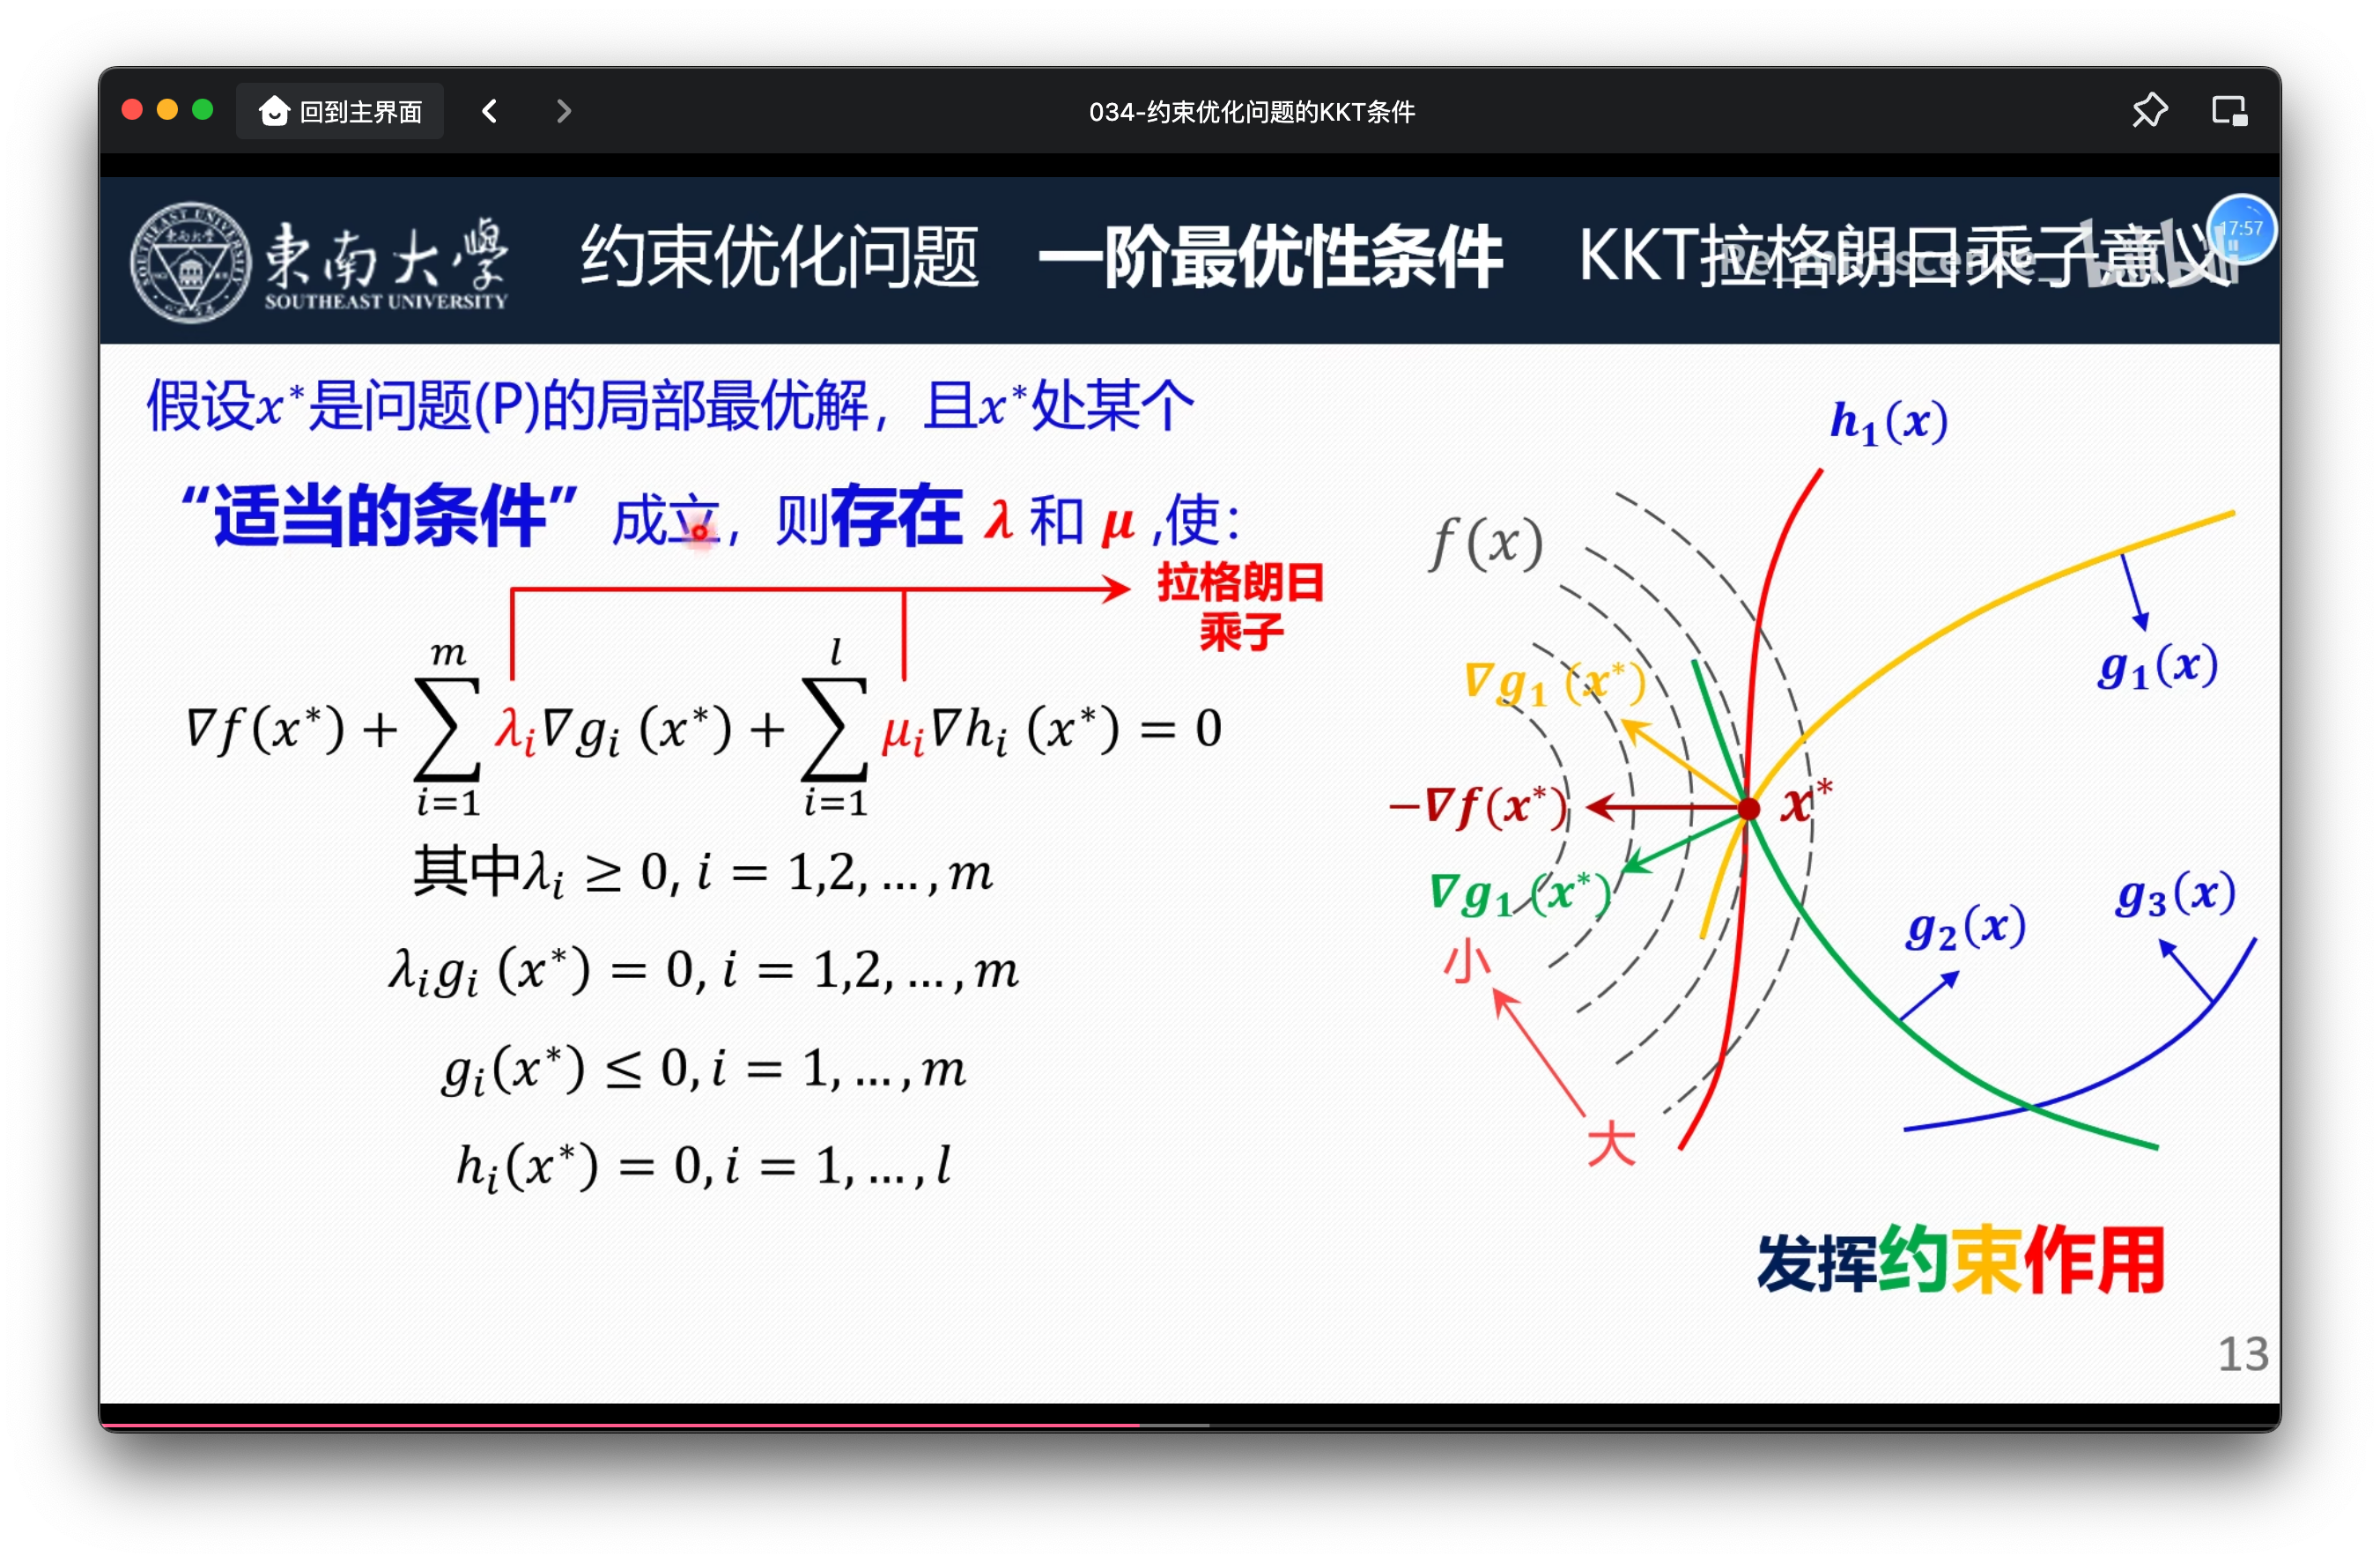
\includegraphics[width=0.50\linewidth]{notes/assets/image-20260107150812169.png}
\end{center}

\begin{center}
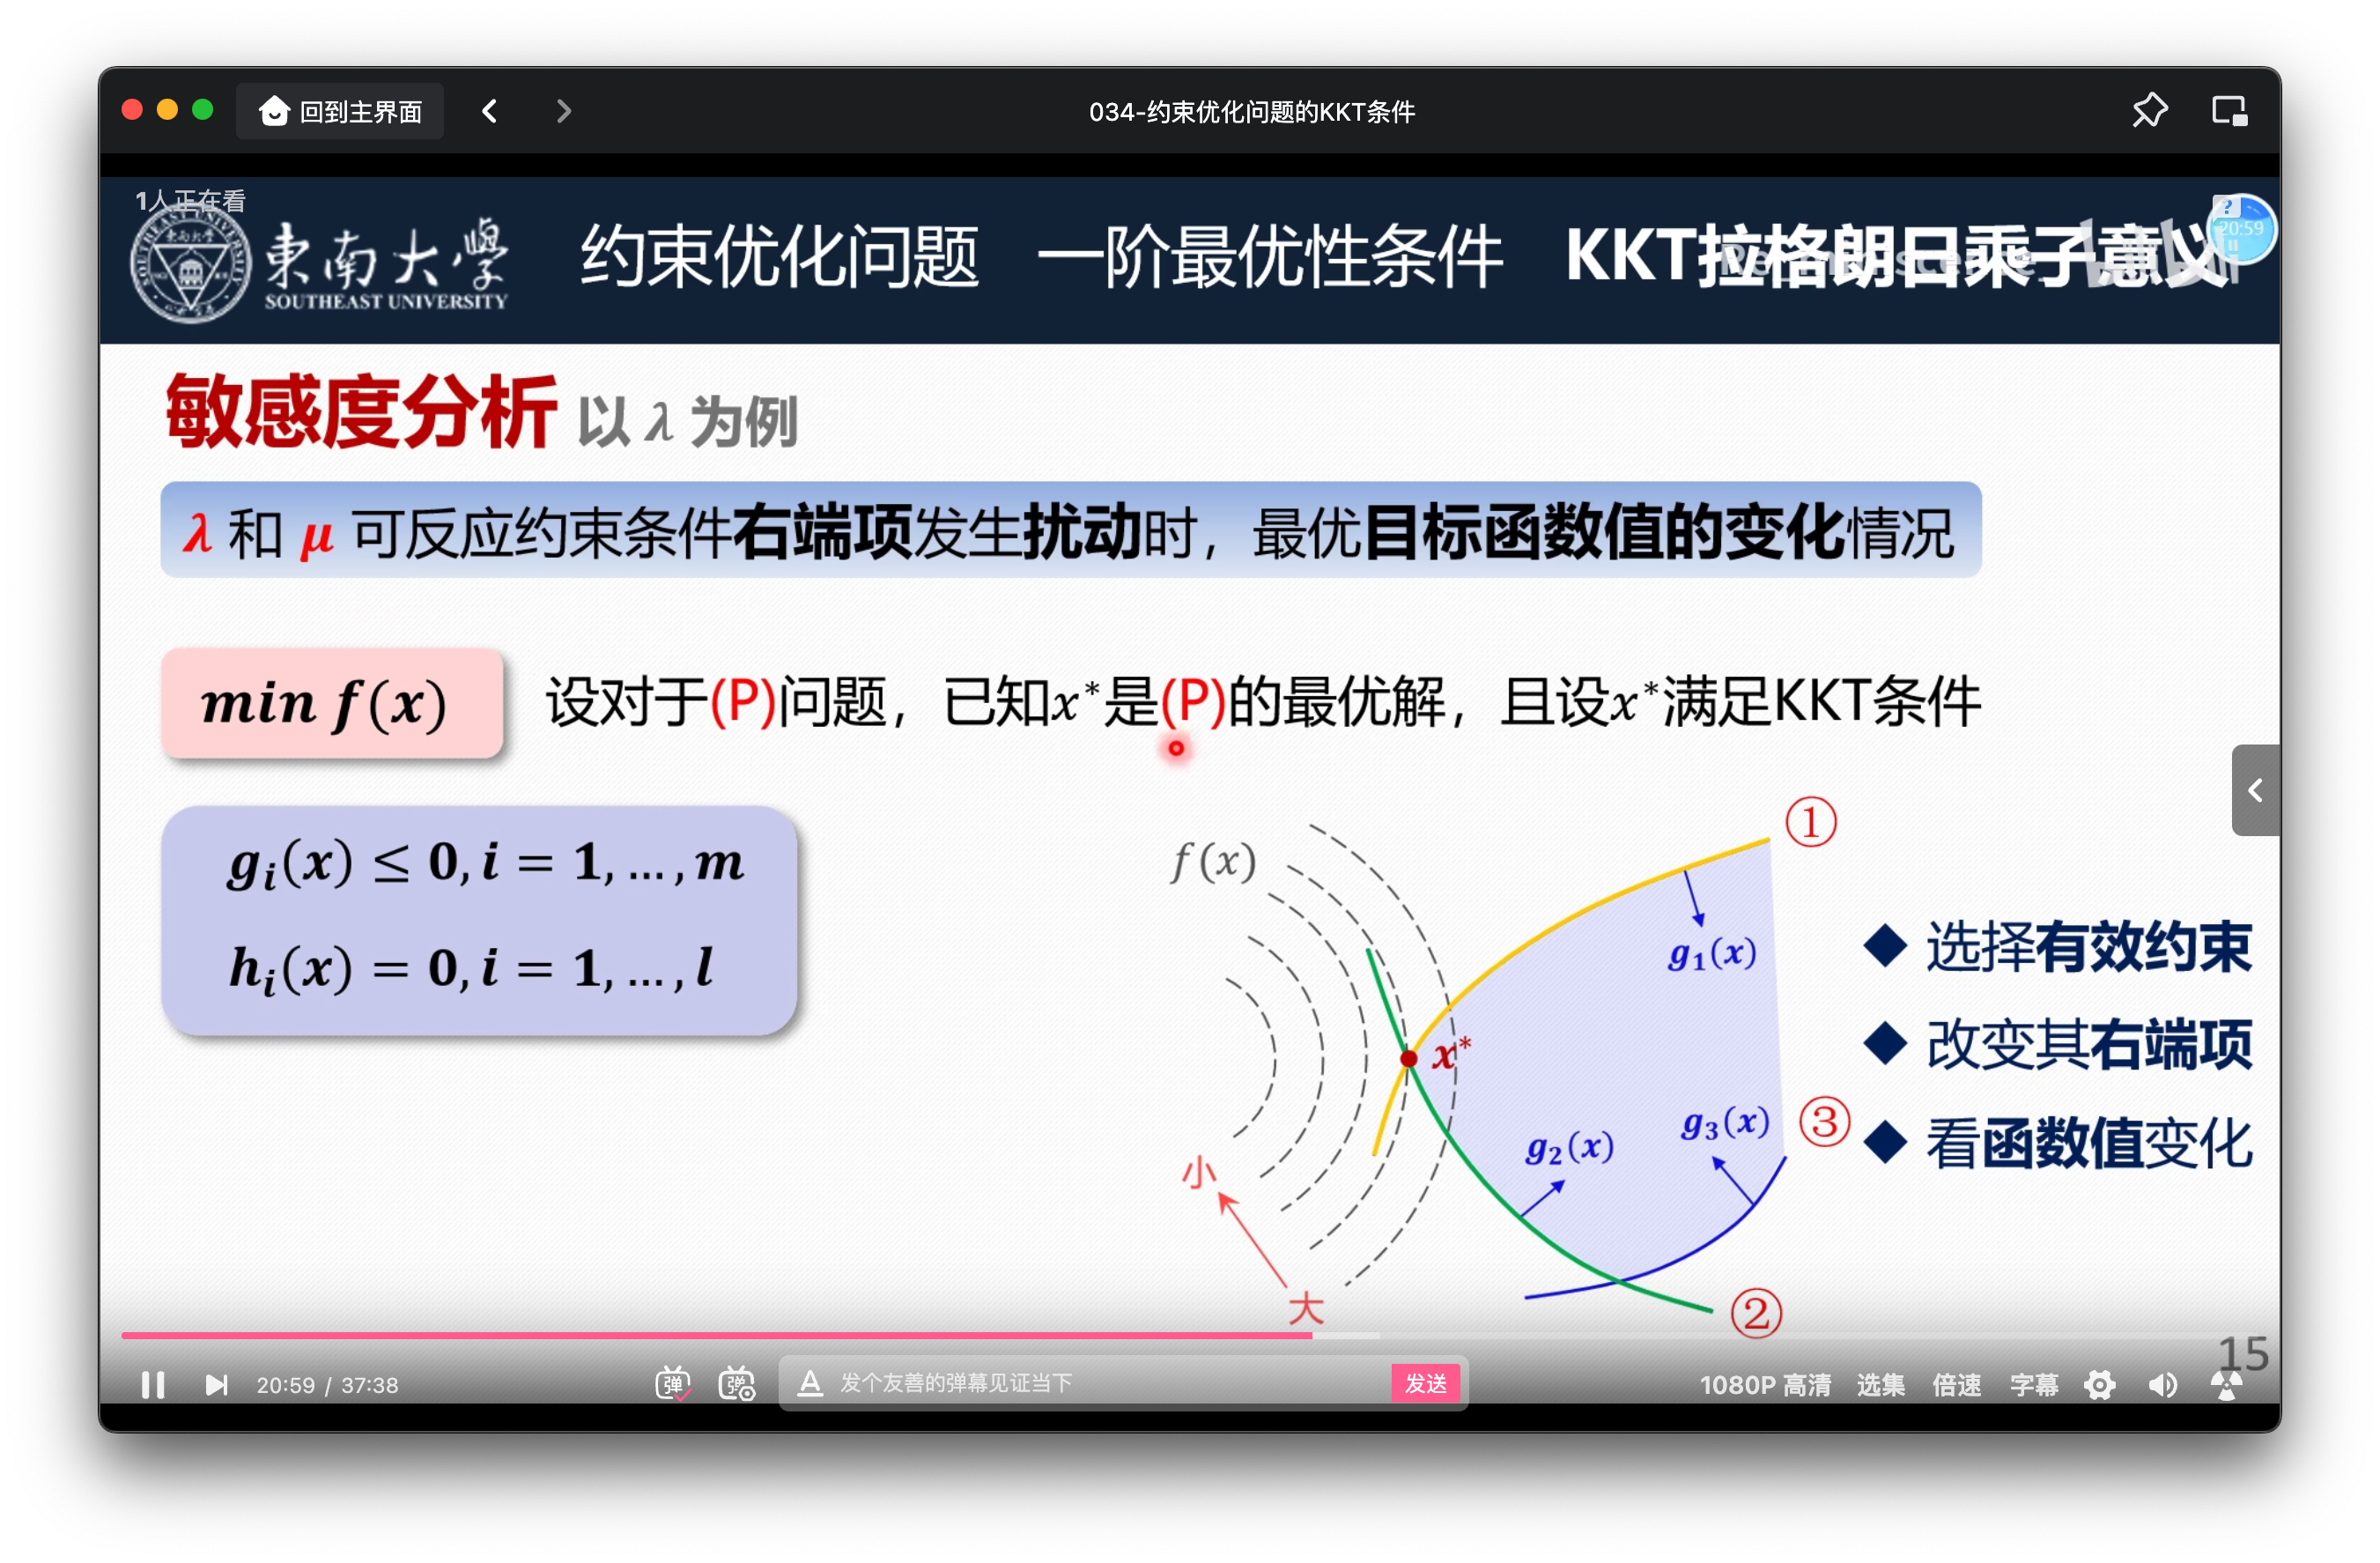
\includegraphics[width=0.50\linewidth]{notes/assets/image-20260107151122909.png}
\end{center}

\begin{center}
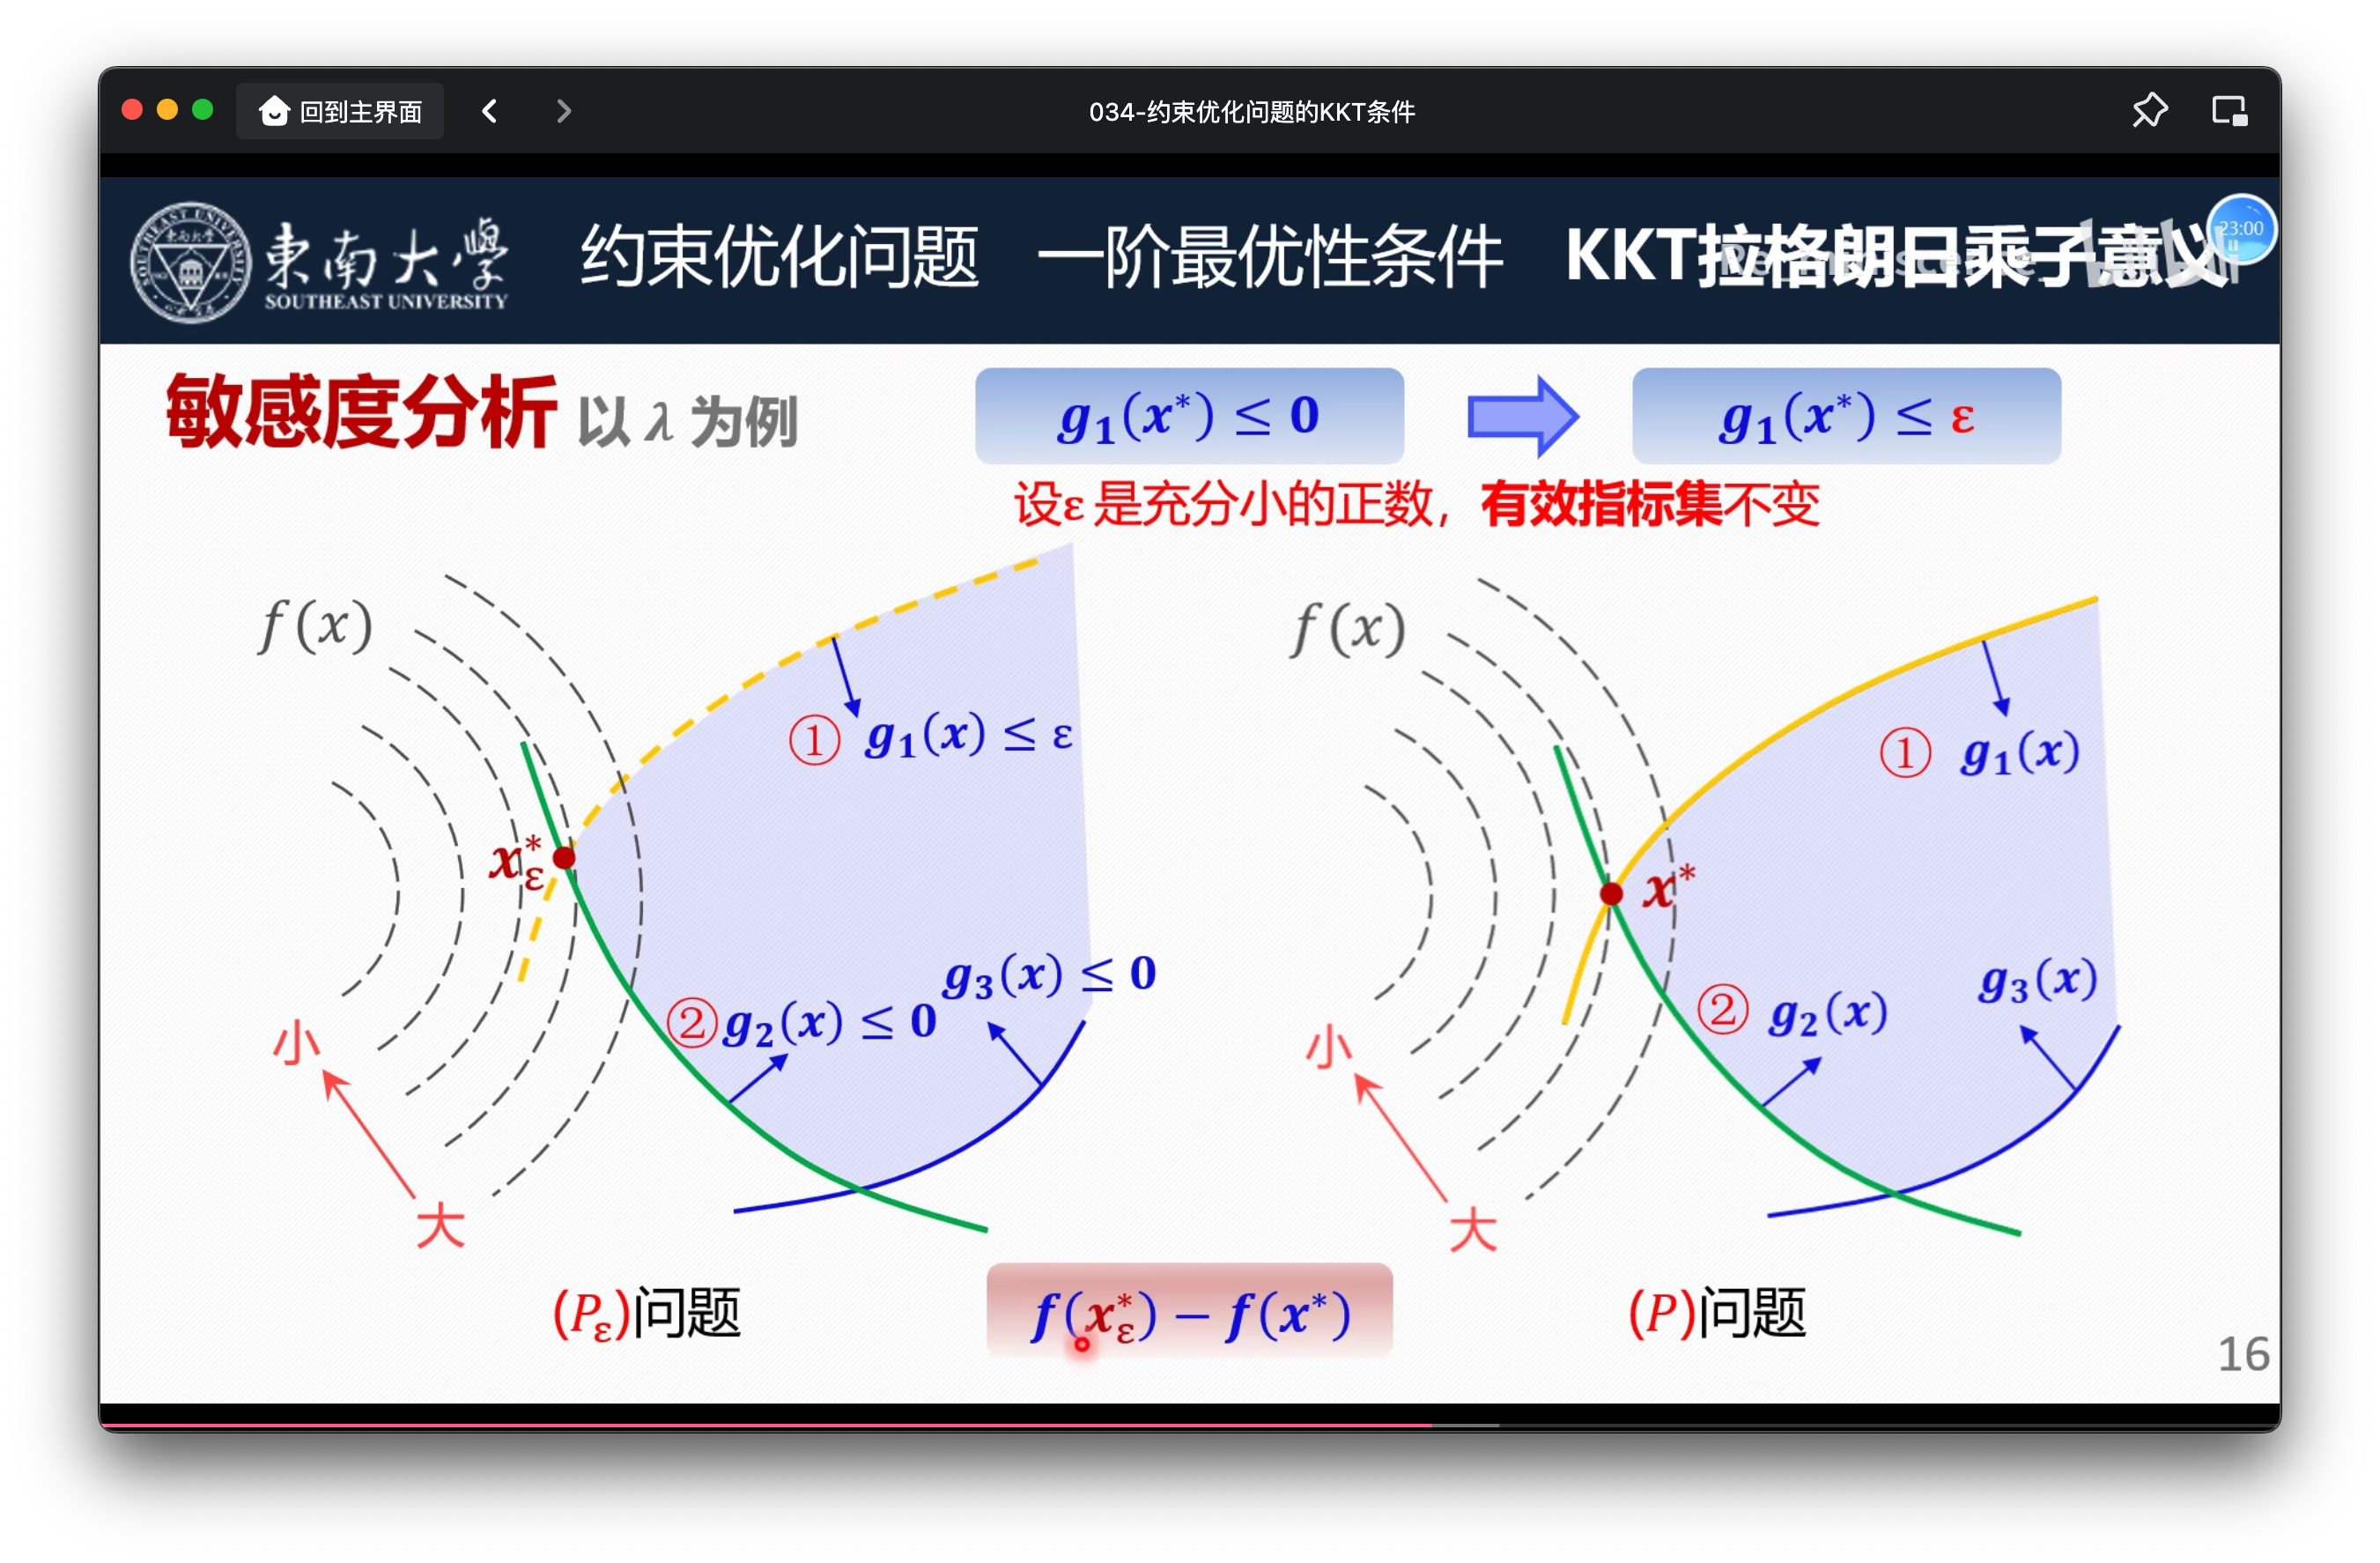
\includegraphics[width=0.50\linewidth]{notes/assets/image-20260107151259853.png}
\end{center}

\begin{center}
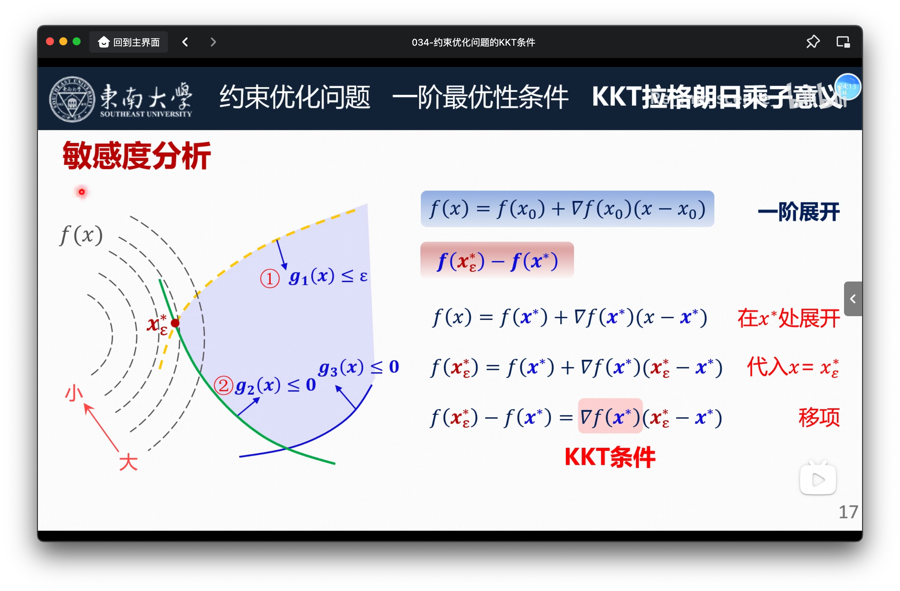
\includegraphics[width=0.50\linewidth]{notes/assets/image-20260107151500816.png}
\end{center}

\begin{center}
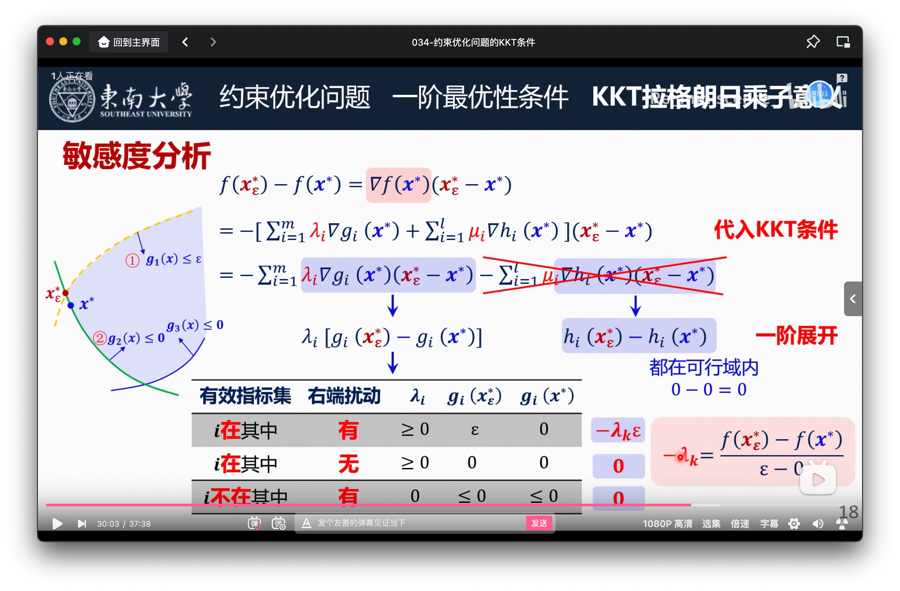
\includegraphics[width=0.50\linewidth]{notes/assets/image-20260107153400164.png}
\end{center}

\begin{center}
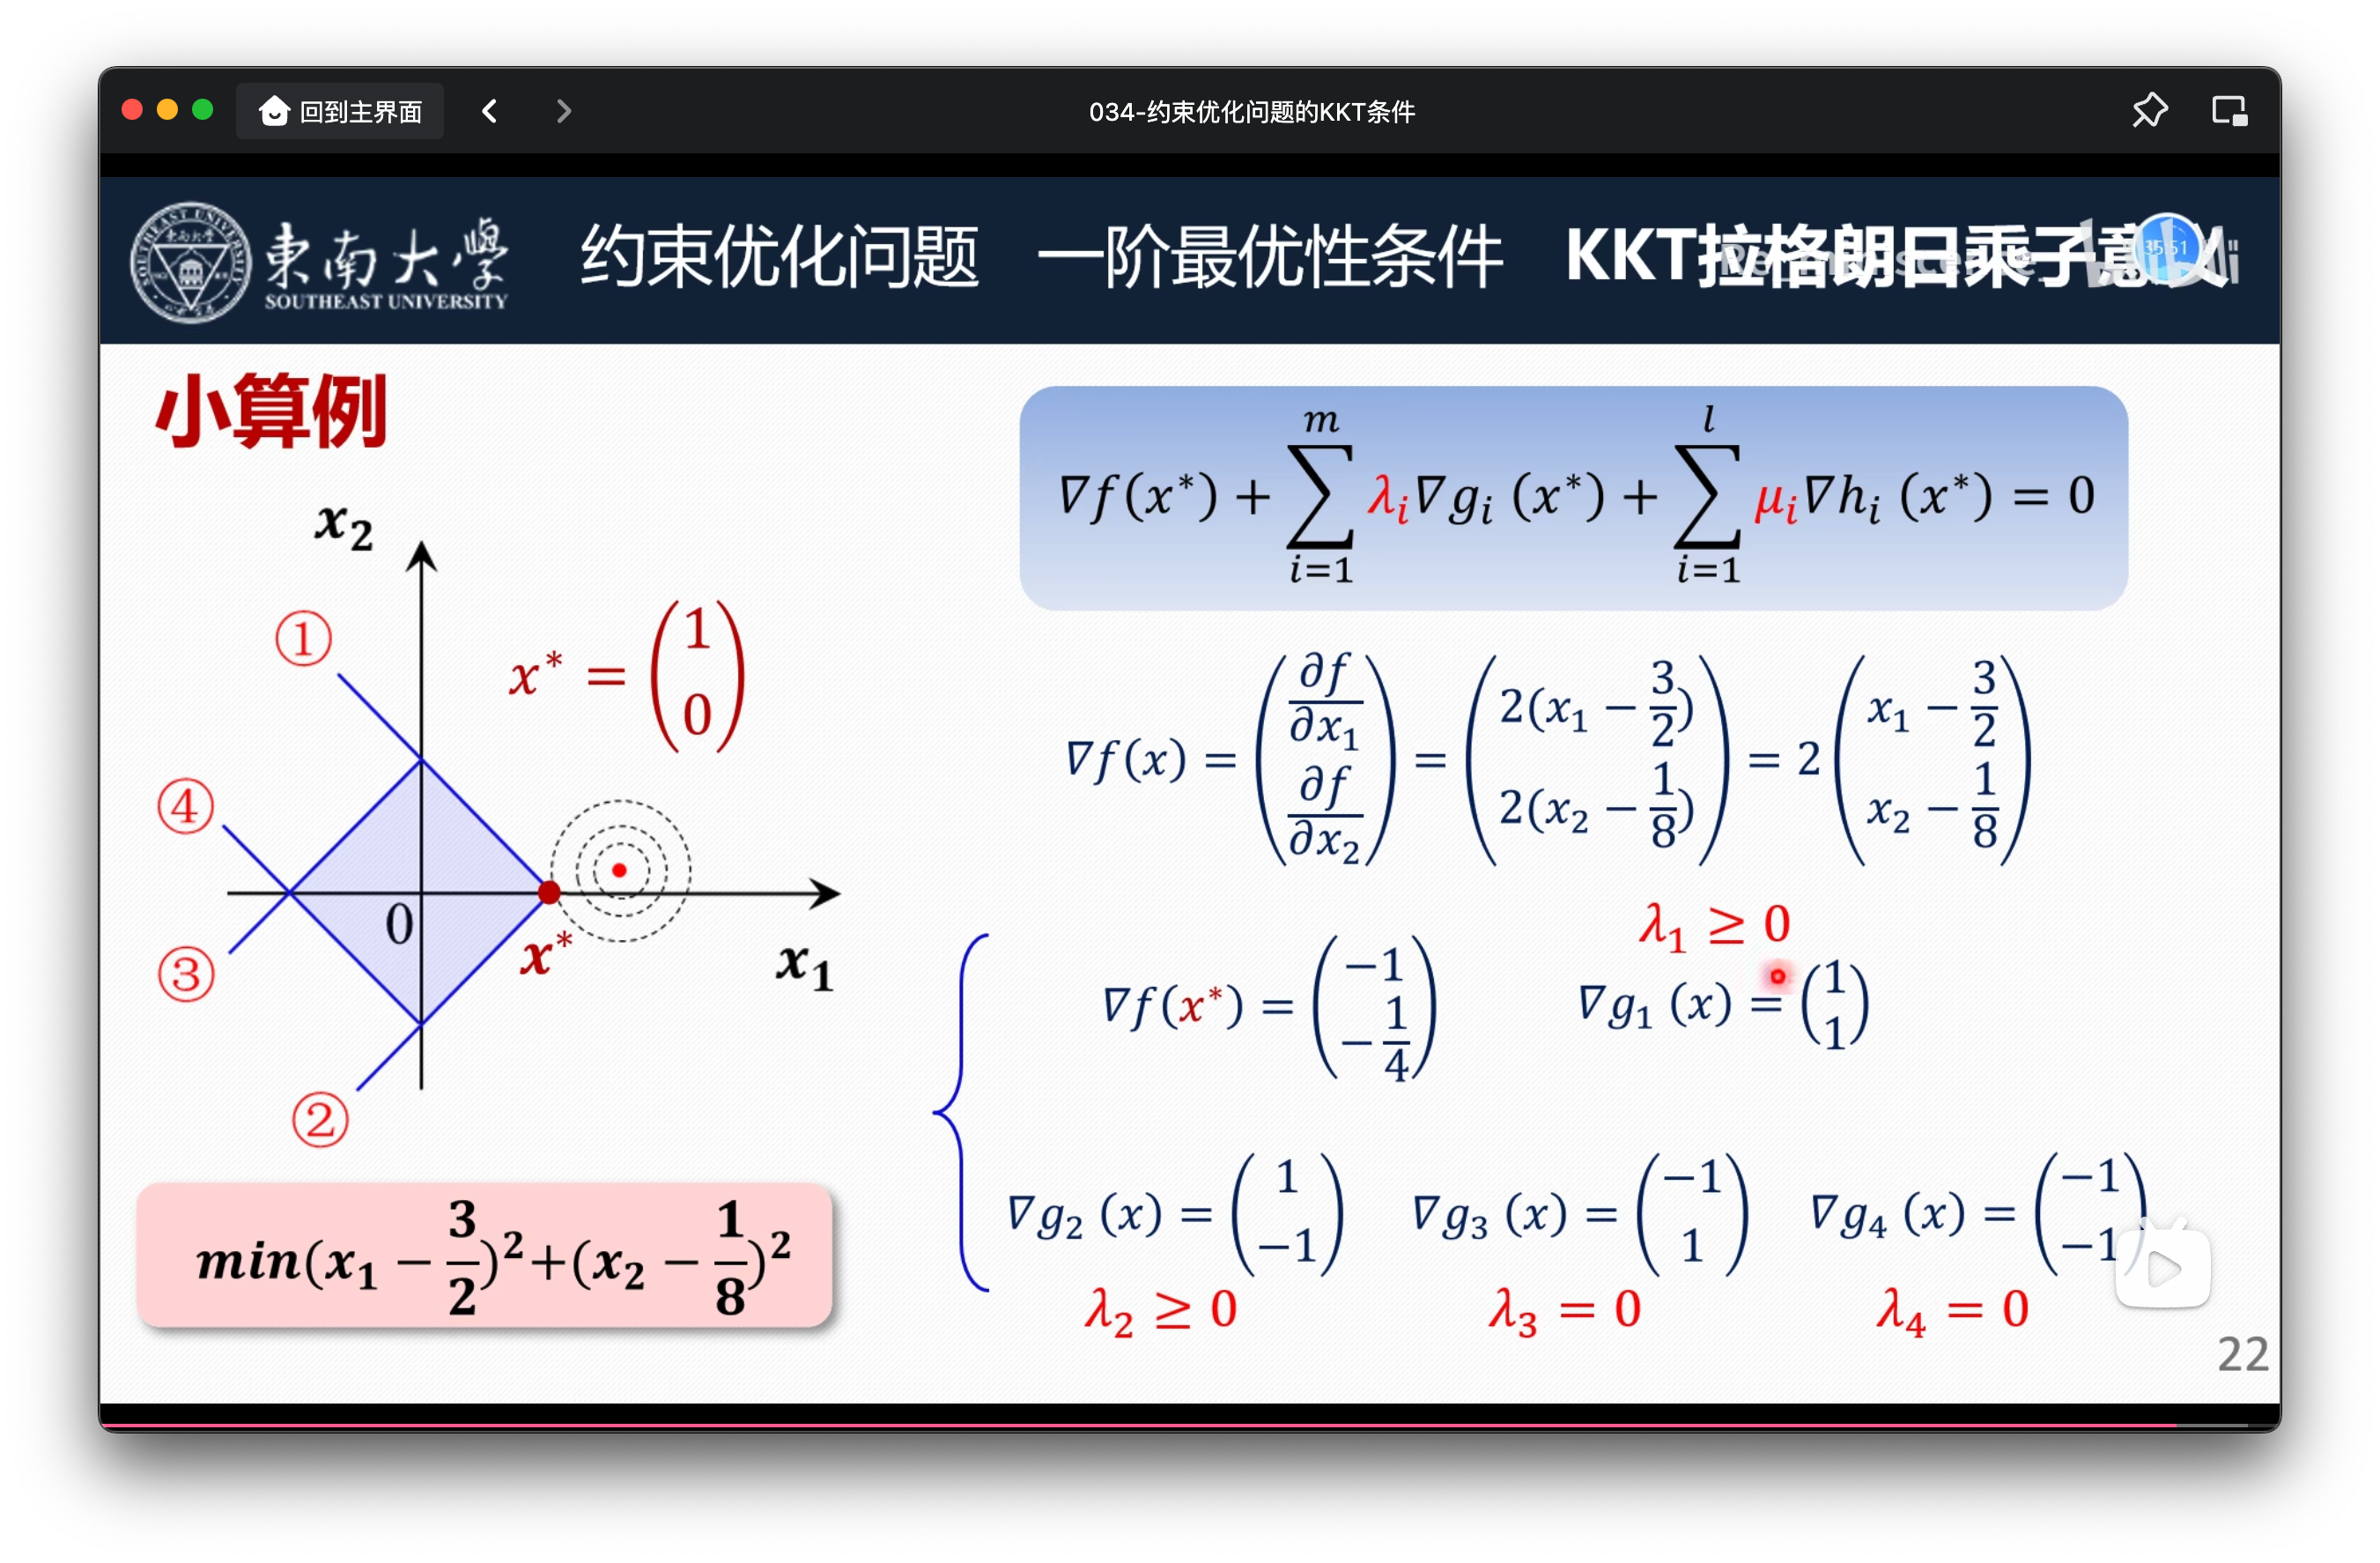
\includegraphics[width=0.50\linewidth]{notes/assets/image-20260107154039642.png}
\end{center}

\begin{center}
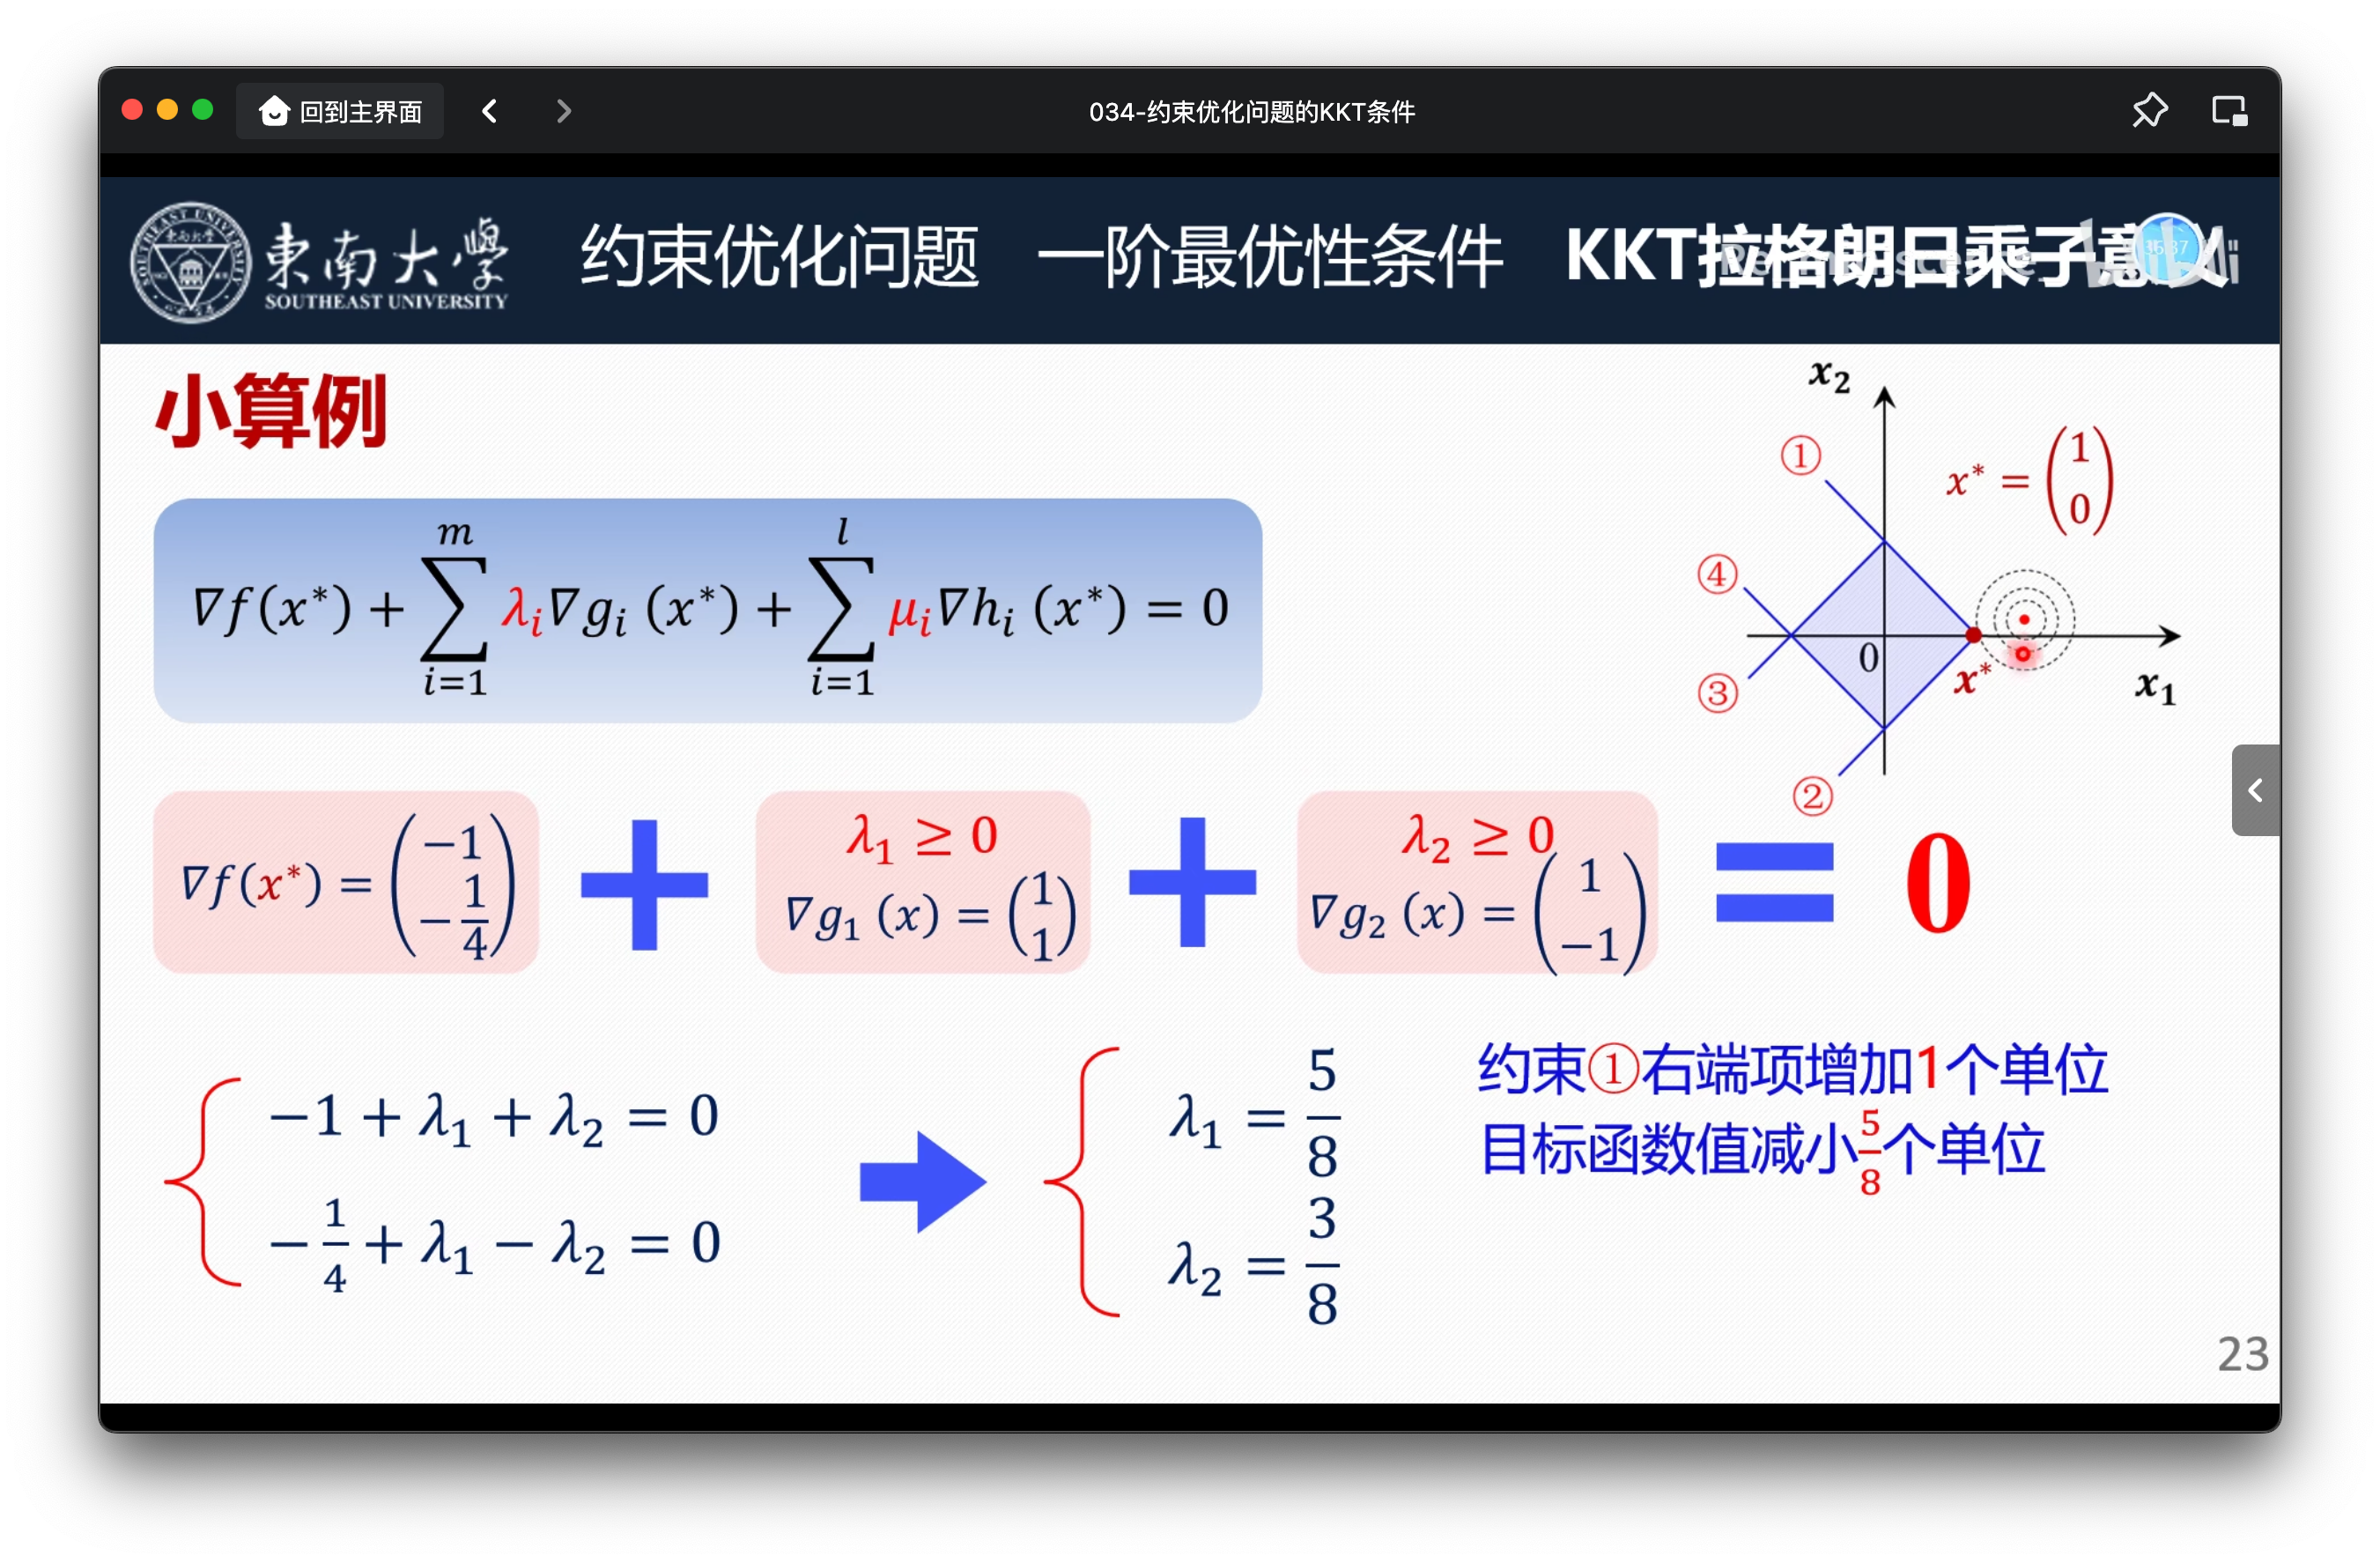
\includegraphics[width=0.50\linewidth]{notes/assets/image-20260107153945202.png}
\end{center}
